% main.tex
% Universitaire Papers - Full Documentation & Usage Guide
% Author: Matt
% Purpose: A self-contained manual that explains paperSettings.tex,
%          standardCommands.tex and demonstrates how to use the macros.
%
% Save this file as main.tex in the root of the repo alongside:
%   - paperSettings.tex
%   - standardCommands.tex
%   - main.bib
%
% Compile with: buildLatexDocument.sh (or fullBuild.sh)
% Or upload to Overleaf and compile there.
% -----------------------------------------

% ----------- Document settings -----------
\documentclass[nonacm, sigconf, balance=true]{acmart}
\include{core/paperSettings} % import custom general paper settings
\include{core/standardCommands} % import custom commands and packages
% -----------------------------------------
\begin{document}

    \onecolumn

    \section{Propositielogica}
    Propositielogica is de studie van bewijzen.
    Een propositie is te beantwoorden met waar of niet waar
    Een propositie is $3 < 17$, dit kan je checken op waarheid.
    Een propositie is $x \implies y$.

    Propositielogica komt ook met een hele hoop termen, zo heb je \textbf{negatie} wat (gezien in een waarheidstabel) het omdraaien van waarde betekend, waar wordt onwaar en vice versa.
    Je hebt ook \textbf{conjunctie}, wat een chique woord is voor \textit{en}, $a \land b$, b EN a.
    Een andere variant is \textbf{disjunctie}, wat dan staat voor \textit{of}, $a \lor b$, a OF b.
    \textbf{Implicatie} is de er ook een, dat is de $x \implies y$, a IMPLCIEERT b.
    De allerlaatste is \textbf{equivalentie}, $a \Leftrightarrow b$, a is equivalent aan b.
    LET OP! Dit betekend niet ``gelijk aan'' 2 rode canta's zijn equivalent, maar niet hetzelfde, het is namelijk niet letterlijk dezelfde auto, maar ze zijn wel identiek aan elkaar.

    \subsection{Proposities}
    We gebruiken in logica variabelen zoals P en Q, dit zijn \textit{atomisch} proposities, deze zijn altijd geschreven in HOOFDLETTERS.
    Deze zijn niet verder op te delen, dus niet opgebouwd van kleinere delen zoals implicaties etc. deze waardes zijn Waar/True/1 of Onwaar/False/0.

    Je hebt ook kleine letters p, q, \ldots, dit zijn niet-atomische proposities, het zijn geen propositionele formules, maar eerder \textit{metavariabelen}.

    \begin{multicols}{2}

        Elke propositionele formule bestaat uit:
        \begin{itemize}
            \item Atomitsche proposities (P, Q, R, \ldots)
            \item true, (T, Waar, 1)
            \item false, (F, Onwaar, 0)
        \end{itemize}

        Deze kunnen ook kleiner opgedeeld zijn, dan zijn dit ook propositionele formules:
        \begin{itemize}
            \item $P \implies Q$ - \textbf{implicatie} als P, dan Q
            \item $P \land Q$ - \textbf{conjunctie} P én Q
            \item $P \lor Q$ - \textbf{disjunctie} P of Q
            \item $\neg P$ - \textbf{negatie} (niet P / P houd geen stand)
        \end{itemize}

    \end{multicols}

    Zoals in de wiskunde ook is heeft propositielogica óók een volgorde, deze is:
    \begin{enumerate}
        \item Haakjes ()
        \item Negatie $\neg$
        \item Conjunctie $\land$
        \item Disjunctie $\lor$
        \item Implicatie $\implies$
    \end{enumerate}

    $\neg P \lor Q \implies Q \land P$ moet gelezen worden als $((\neg P) \lor Q) \implies (Q \land P)$

    Om dit te onthouden kan je deze zij onthouden: ``Hoe Navigeert Connie De Ijssel''

    \subsection{Semantiek van propositie operatoren}

    \begin{SimpleTable}[s{.3}s{.3}s{.3}s{.3}s{.3}s{.3}s{.3}s{.3}s{.3}]{Truthtable van basisoperaties}{}
        \TableHeader{$P$ & $Q$ & $\neg P$ & $P \land Q$ & $P \lor Q$ & $P \oplus Q$ & $P \implies Q$ & $P \equiv Q$}
        \TableRow{0 & 0 & 1 & 0 & 0 & 0 & 1 & 1}
        \TableRow{0 & 1 &   & 0 & 1 & 1 & 1 & 0}
        \TableRow{1 & 0 & 0 & 0 & 1 & 1 & 0 & 0}
        \TableRow{1 & 1 &   & 1 & 1 & 0 & 1 & 1}
    \end{SimpleTable}

    Maar stel, je wilt iets moeilijks bewijzen zoals $\neg P \lor Q \implies Q \land P$, dan kan je dat op de volgende manier doen:

    \vsmall

    \begin{SimpleTable}[s{.3}s{.3}s{.3}s{.3}s{.3}s{.3}]{Truthtable van moeilijkere propositie formule}{}
        \TableHeader{$P$ & $Q$ & $\neg P$ & $\neg P \lor Q$ & $ Q \land P$ &  $\neg P \lor Q \implies Q \land P$}
        \TableRow{0 & 0 & 1 & 1 & 0 & 0}
        \TableRow{0 & 1 & 1 & 1 & 0 & 0}
        \TableRow{1 & 0 & 0 & 0 & 0 & 1}
        \TableRow{1 & 1 & 0 & 1 & 1 & 1}
    \end{SimpleTable}

    Je kan ook met verschillende kleuren pennen een kleine waarheidstabel schrijven, maar dit is een hele nette manier om het ook te doen.

    \subsection{Voorbij thruth tables}
    Je kan d.m.v een truth table bewijzen of een formule wel of niet houd, maar dat kan ook anders, bijvoorbeeld door het versimpelen van de formules.

    \begin{SimpleTable}[s{.1}s{.5}s{.4}]{}{}
        \TableHeader{ & Expression & Law}
        \TableRow{                  & $(p \implies q) \lor (q \implies p)$      & original}
        \TableRow{$\Leftrightarrow$ & $(\neg p \lor q) \lor (\neg q \lor p)$    & implication}
        \TableRow{$\Leftrightarrow$ & $\neg p \lor ((q \lor \neg q) \lor p)$    & associativity / rearrangement}
        \TableRow{$\Leftrightarrow$ & $\neg p \lor (T \lor p)$                  & tertium non datur}
        \TableRow{$\Leftrightarrow$ & $\neg p \lor T$                           & absorbing property of \(T\)}
        \TableRow{$\Leftrightarrow$ & $T$                                       & absorbing property of \(T\)}
    \end{SimpleTable}


    Mocht het nou gebeuren dat elke rij waar is, ofwel de combinatie van input waardes maakt niet uit voor de uitkomst; deze is altijd waar.
    Dan heet dat een \textbf{tautologie}.
    Voor het omgekeerde (altijd onwaar), geld dat dit een \textbf{contradictie} heet.
    
    Deze afleiding kan je maken door de regels te gebruiken die hieronder stan geschreven (er zijn er nog meer).

    \begin{multicols}{3}

        Commutativity:
        \begin{itemize}
            \item $p \land q \Leftrightarrow q \land p$
            \item $p \lor q \Leftrightarrow q \lor p$
        \end{itemize}

        Associativity:
        \begin{itemize}
            \item $p \land (q \land r) \Leftrightarrow (p \land q) \land r$
            \item $p \lor (q \lor r) \Leftrightarrow (p \lor q) \lor r$
        \end{itemize}

        Tertium non datur:
        \begin{itemize}
            \item $p \lor \neg p \Leftrightarrow T$
        \end{itemize}

        Idempotence:
        \begin{itemize}
            \item $p \land p \Leftrightarrow p$
            \item $p \lor p \Leftrightarrow p$
        \end{itemize}

        De Morgan:
        \begin{itemize}
            \item $\neg (p \lor q) \Leftrightarrow \neg p \land \neg q$
            \item $\neg (p \land q) \Leftrightarrow \neg p \lor \neg q$
        \end{itemize}

        Double negation (niet niet is wel):
        \begin{itemize}
            \item $p \Leftrightarrow \neg(\neg p)$
        \end{itemize}

        Properties of T en F:
        \begin{itemize}
            \item $p \lor F \Leftrightarrow p$
            \item $p \land F \Leftrightarrow F$
            \item $q \lor T \Leftrightarrow T$
            \item $q \land T \Leftrightarrow q$
        \end{itemize}

        Implication:
        \begin{itemize}
            \item $(p \implies q) \Leftrightarrow (\neg p \lor q)$
        \end{itemize}

        Contraposition:
        \begin{itemize}
            \item $(p \implies q) \Leftrightarrow (\neg q \implies \neg p)$
        \end{itemize}

    \end{multicols}

    \section{sets}
    Propositielogica heeft ook een manier om over een groep dingen te redeneren, \textit{\textbf{sets}}.
    Deze schrijf tussen accolades met comma's tussen de items: $\{ false, true \}$, $\{ 3, 7, 14 \}$, $\{ red, blue, yellow\}$.
    Dit kan voor kleine sets met de hand, maar als je grote sets wilt schrijven, dan kost dat heel veel tijd, daarom kan je ook: ${ 1, 3, 5, ..., 99}$ om alle oneven cijfers van 1 t/m 99 als set te hebben.
    Of als ${1, 2, 3, ...}$ om alle cijfers vanaf 1 te hebben (oneindig).
    De lengte van een sets is op te schrijven door |A| of #A, waar A een set is met een lengte, de \textbf{cardinality} hier tel je alleen het aantal unieke elementen, maar dit werkt alleen voor eindige sets, dus $|{1,2,3,4}| = 4$.
    Als er maar 1 element in een set zit, dan heet dat een \textbf{singleton}.

    Ook kan je de \textit{\textbf{set-builder notation}} gebruiken, hierbij schrijf je het soort element dat je wilt en wat het element kan zijn:
    $\{\text{x : x has the property P}\}$

    \begin{voorbeeld}{Set-builder notation}
        Een collectie van alle prime numbers: $\{\text{x : x is een priemgetal}\}$\\
        Of $\{\text{s : s is een strand in Nederland}\}$.
    \end{voorbeeld}

    Er zijn ook een paar basis sets, die al van tevoren zijn gedefinieerd:

    \begin{itemize}
        \item $\emptyset = \{ \}$ & (the empty set)
        \item $\mathbb{B} = \{ 0, 1 \} $ & (the binaire set)
        \item $\mathbb{N} = \{ 0, 1, 2, 3, ... \}$ & (De natuurlijke nummers)
        \item $\mathbb{Z} = \{ ..., -2, -1, 0, 1, 2, ... \}$ & (De integers)
        \item $\mathbb{Q} = \{\dfrac{m}{n} : \text{m, n} \in \mathbb{Z} \text{, n} \neg \text{0} \}$ & (De rationele nummers)
        \item $\mathbb{R} =  \{ x : \text{x is a real number} \}$ & (De real nummers)
    \end{itemize}

    \textbf{$\emptyset$ en \{ $\emptyset$ \} zijn twee verschillende dingen, de een is namelijk: \{ \}, terwijl de ander \{ \{ \} \} is!}

    \subsection{leden en gelijkheid}
    Je kan bekijken of een set een bepaalde member heeft door $7 \in \{3,7,14\}$ te doen.
    Hier is $\in$ te lezen als \textit{"is element onderdeel van"}
    Je hebt ook de negatie vorm, $\not\in$, wat \textit{"is element niet onderdeel van"}, oftwel $6 \not\in \{3,7,14\}$ betekend.

    Ook is goed om te weten dat gelijkheid op basis van unieke element rust, dus $\{1, 2, 3, 2, 1\} \eq \{1, 3, 2\}$.
    Ongelijkheid is dus te bepalen door te kijken of een van de twee sets een waarde heeft die niet in de ander voorkomt.
    Dus volgorde maakt niet uit, en hoeveelheid elementen die dan welniet hetzelfde zijn maakt ook niet uit.

    \subsection{subsets and supersets}
    Een \textit{\textbf{subset}} is een set waarin minstens een deel van de waardes van de superset in voorkomen.

    \begin{multicols}{2}
        Dus $A = \{1, 2, 3\}$ is een subset van $B = \{1, 2, 3, 4\}$, hierin is B een \textit{\textbf{superset}} van A en A een \textit{\textbf{subset}} van B
        Dit schrijf je als volgt: $A \subseteq B$ \textit{(A is included or contained in B)} en vice versa $B \supseteq A$ \textit{(B includes or contains A)}.

        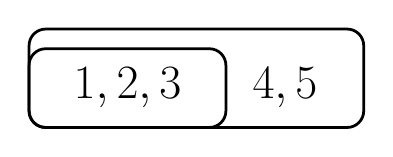
\begin{tikzpicture}
            \tikzstyle{every node}=[font=\LARGE]
            \draw [ line width=1pt , rounded corners = 6.0] (3,9) rectangle (7.25,7.75);
            \draw [ line width=1pt , rounded corners = 6.0] (3,8.75) rectangle (5.5,7.75);
            \node [font=\LARGE] at (4.25,8.25) {$1, 2, 3$};
            \node [font=\LARGE] at (6.25,8.25) {$4, 5$};
        \end{tikzpicture}

    \end{multicols}

    \subsection{Operaties op sets}
    Union $A \cup B = \{x : x \in A \lor x \in B \}$ Combineert A en B met elkaar\\
    Intersection $A \cap B = \{x : x \in A \land x \in B\}$ Het deel wat zowel in A als in B zit\\
    Complement $\overline{A} = \{x : x \not\in A\}$, alles wat niet in A zit.\\
    Difference $A\B = \{x: x \in A \land X \not\in B\}$ Alles wat in A zit, maar niet in B\\

    Zo heb je ook de \textit{powerset P(A)}, dit is een set waarin alle mogelijke subsets van A zitten: $P(A) = \{ X : X \subseteq A \}$.
    Deze heeft $n^2$ elementen, waar n het aantal elementen van set A is.

    \begin{voorbeeld}{powerset/matchsset}
        Stel je hebt een computer scherm, van 1680 x 1050, je wilt elke mogelijke configuratie van zwart/witte pixels opschrijven.
        Een set geeft aan welke pixels wit zijn, dus je wilt elke set met elke mogelijke manier van pixelcoordinaten, dat kan je zo schrijven:

        $W = \{0,1, ..., 1697\}$ voor elke X coordinaat\\
        $H = \{0,1,...,1049\}$ Voor elke Y coordinaat\\
        $W\times H = \{\{0,0\}, \{0,1\}, \{0,2\},...,\{1,0\},...\{1679,1049\}\}$ dit is een volledig wit scherm, elke pixel is gerepresentateerd in deze set\\
        $P(W\times H)$ = elke configuratie van witte pixels
    \end{voorbeeld}

    \subsection{Partities}
    Je kan een set A opdelen in meerdere sets, zoals $A_1$ en $A_2$, hier zijn de regels: $A_1 \cup A_2 = A$ en $A_1 \cap A_2 = \emptyset$
    Zo kan je A = $\mathbb{N}$ opsplitsen in $A_1$ en $A_2$ waar $A_1$ de even getallen zijn en $A_2$ de oneven getallen zijn.

    \subsection{Naive set theory}
    %TODO


    \section{Boolean algebra}
    korte notitie* in Bolean algebra is de $+$ hetzelfde als de OR operator, $\cdot$ hetzelfde als de AND operator, $^{-1}$ hetzelfde als NOT

    \subsection{monoïde}
    Monoide is een verzameling A, is niet ledig en heeft minstens 1 element e, en een binaire operator $\oplus$ %TODO: verder uitschrijven
    Een monoide heeft een nul-element, dit is een waarde die niks doet in de operatie. $x + 0 = x$, hier doet de 0 helemenaal niks, dus 0 is het 0-element in de "+" operatie.
    $x \times 1 = x$, hier is 1 het nul-element in de monoide $\times$ 1; het doet niks in de operatie.
    het is dus een neutrale waarde.

    \subsection{Bool's algebra}

    Boolean algebra heeft een paar regels:

    \begin{itemize}
        \item een set B
        \item Twee elementen $0 \in B$ en $1 \in B$, genaamd \textbf{zero} en \textbf{unit}
        \item Twee binaire operatoren $+$ en $\cdot$ som/OR en product/AND respectievelijk.
        \item Een Unaire operator $^{-1}$ de inverse genoemd ofwel NOT (kan ook als $x'$ zijn genoteerd).
    \end{itemize}

    \begin{voorbeeld}{Bewijs dat $x + x = x$}
        We willen bewijzen dat voor elke $x, x + x = x$\\
        \begin{SimpleTable}[s{.3}s{1}s{.3}]{}{}
            \TableRow{$x + x$ & $= (x + x) \cdot 1$               & Ident}
            \TableRow{        & $= (x + x)\cdot (x \cdot x^{-1})$ & Complement}
            \TableRow{        & $= x + (x \cdot x^{-1})$          & Distrobution}
            \TableRow{        & $= x + ()$                        & Complement}
            \TableRow{        & $= x$                             & Ident}
        \end{SimpleTable}
    \end{voorbeeld}

    \subsection{dualiteit}
    Je kan voor elke vergelijking die je opschrijft een soort duale tweede vergelijking maken door hetvoglende te doen:

    \begin{itemize}
        \item 0 met 1 vervangen
        \item 1 met 0 te vervangen
        \item $+$ met $\cdot$ te vervangen
        \item $\cdot$ met $+$ te vervangen
    \end{itemize}

    \subsection{waarheidstabel naar formule/circuit}
    Stel je krijgt een waarheidstabel zoals deze:

    \begin{multicols}{2}
        \begin{SimpleTable}[s{.3}s{.3}s{.3}]{}{}
            \TableHeader{$x$ & $y$ & $z$}
            \TableRow{0 & 0 & 0}
            \TableRow{0 & 1 & 1}
            \TableRow{1 & 0 & 1}
            \TableRow{1 & 1 & 0}
        \end{SimpleTable}

        Als je dit omzet naar een propositie, dan moet je kijken naar alle rijen waar de uitkomst 1 is.
        Voor elke 0 waarde schrijf je de variabele (hier x of y), op als $\overline{x}\text{ of }\overline{y}$.
        Elke 1 waarde schrijf je alleen de variabele op, dus x of y.
        Als je dat hier zou doen dan krijg je hetvolgende antwoord: $(\overline{x} \land y) \lor (x \land \overline{y})$.
        Dit kan je dan vervolgens omzetten naar een circuit:
    \end{multicols}

    \begin{figure}[h]
        \raggedright
        \includegraphics[width=40mm]{images/boolean_circuit}
    \end{figure}


    \newpage


    \section{Predikatenlogica}

    \subsection{Predicaten en vrije variabelen}

    We zagen eerder de \textit{set-builder}-notatie
    \[
        \{x \mid x \text{ heeft eigenschap } P\},
    \]
    waarbij \(P\) een voorwaarde is. Een voorbeeld van zo’n voorwaarde is
    \[
        P(x) = Prime(x) = \text{``$x$ is een priemgetal''}.
    \]
    Het predicaat geeft voor elke waarde \(x\) waar of onwaar terug, en op basis daarvan bepalen we of \(x\) tot de verzameling behoort. De bijbehorende \textit{truth set} bestaat uit alle waarden die voldoen aan het predicaat.

    \begin{voorbeeld}{Eendjes}
        We hebben zeven eendjes:
        \[
            Eendjes = \{Kwik, Kwek, Kwak, Dagobert, Donald, Katrien, Dumbella\}.
        \]

        We definiëren het predicaat
        \[
            Female(x) = \text{``$x$ is vrouwelijk''}.
        \]

        \begin{itemize}
            \item \(Female(Katrien) \land Female(Dumbella)\) is waar.
            \item \(Female(Kwik) \land Female(Kwek) \land \dots \land Female(Donald)\) is niet waar.
            \item De truth set van \(Female(x)\) is dus \(\{Katrien, Dumbella\}\).
        \end{itemize}
    \end{voorbeeld}

    \subsection{Kwantificatoren en gebonden variabelen}

    Stel dat we willen controleren of elke waarde in een lijst aan een voorwaarde voldoet. Het boek geeft het volgende voorbeeld:

    Er zijn vier kinderen:
    \[
        Kinderen = \{Joel, Felix, Oskar, Amanda\}.
    \]

    Eén van hen moet voorin op de passagiersstoel zitten, omdat er achterin maar drie plekken zijn. Het predicaat \(Front(x)\) betekent dat kind \(x\) voorin zit. We weten dus zeker dat voor één waarde van \(x\) het predicaat waar moet zijn.

    De samengestelde propositie
    \[
        Front(Joel) \lor Front(Felix) \lor Front(Oskar) \lor Front(Amanda)
    \]
    moet waar zijn. Dat levert in principe een grote lijst aan mogelijke combinaties op, wat snel onoverzichtelijk wordt.
    \\
    \\
    Als je een predikaat schrijft zoals $P(x) = \dots x \dots$, dan is x een gebonden variabele.
    Als je een predikaat schrijft zoals $P(x) = \dots y \dots$, dan is y een vrije variabele.\\
    Bij gebonden variabelen kan je de x vervangen door een waarde, $P(x) = x > 1337$. $P(10000)$ wordt dan $10000 > 1337$

    \subsection{Universele kwantificator}

    Om dit compacter te schrijven gebruiken we de universele kwantor \(\forall\).
    De notatie \(\forall x\, P(x)\) betekent: “voor elke \(x\) geldt \(P(x)\)”.
    De propositie is alleen waar wanneer alle waarden voldoen aan \(P\).

    Het voorbeeld
    \[
        Happy(Joel) \land Happy(Felix) \land Happy(Oskar) \land Happy(Amanda)
    \]
    kun je schrijven als
    \[
        \forall x\, Happy(x),
    \]
    waarbij de vraag is: zijn Joel, Felix, Oskar én Amanda allemaal blij?

    \subsection{Existentiële kwantificator}

    Als je wilt uitdrukken dat er minstens één waarde is waarvoor het predicaat waar is, gebruik je de existentiële kwantor \(\exists\).

    De notatie \(\exists x\, P(x)\) betekent: “er bestaat een \(x\) waarvoor \(P(x)\) geldt”.
    Deze propositie is waar wanneer één of meer waarden voldoen aan \(P\).

    Het voorbeeld
    \[
        Happy(Joel) \lor Happy(Felix) \lor Happy(Oskar) \lor Happy(Amanda)
    \]
    kan worden geschreven als
    \[
        \exists x\, Happy(x).
    \]

    Daarnaast bestaat er de vorm \(\exists! x\, P(x)\):
    “Er bestaat precies één \(x\) waarvoor \(P(x)\) geldt.”

    \subsection{Gebonden kwantificatoren}

    Je kunt kwantoren beperken tot een verzameling.

    De universele, beperkte vorm:
    \[
        \forall x \in A\; P(x)
        \quad\text{(alle waarden in \(A\) voldoen aan \(P\)).}
    \]

    De existentiële, beperkte vorm:
    \[
        \exists x \in A\; P(x)
        \quad\text{(er bestaat minstens één waarde in \(A\) die voldoet aan \(P\)).}
    \]

    \subsection{predikatenlogica lezen}

    \begin{itemize}[leftmargin=*]
        \item \( \forall x\,P(x)\) \quad → \quad ``Voor alle \(x\) geldt: \(P(x)\)''. ``Elke \underline{[type van $x$]} heeft de eigenschap ...''.
        \item \( \exists x\,P(x)\) \quad → \quad ``Er bestaat een \(x\) zodanig dat \(P(x)\)''. ``Er is ten minste één \underline{[type]} waarvoor ...''.
        \item \( \exists! x\,P(x)\) \quad → \quad ``Er bestaat precies één \(x\) zodanig dat \(P(x)\)''. In goed Nederlands: ``Er is precies één ... die/het ...''.
        \item \(P(x)\wedge Q(x)\) \quad → \quad ``\(P(x)\) en \(Q(x)\)''.
        \item \(P(x)\vee Q(x)\) \quad → \quad ``\(P(x)\) en/of \(Q(x)\)''.
        \item \(P(x)\rightarrow Q(x)\) \quad → \quad ``Als \(P(x)\), dan \(Q(x)\)''.
        \item \(\neg P(x)\) \quad → \quad ``niet \(P(x)\)''.
        \item \(x = y\) \quad → \quad ``\(x\) en \(y\) zijn hetzelfde object''.
        \item Meerdere kwantoren: volg strikt de volgorde \(\forall x\exists y\) → ``Voor elke \(x\) bestaat een \(y\) ...'', \(\exists y\forall x\) → ``Er bestaat een \(y\) die voor alle \(x\) ...'' (volgorde verandert betekenis!).
    \end{itemize}

    \begin{voorbeeld}{Een Predikatenlogica formule lezen}
        \[
            \forall x\big( Student(x) \to \exists y( Course(y) \land Enrolled(x,y) \land \neg Failed(x,y))\big).
        \]

        \textbf{Stap 1:} Kies domein = ``personen en vakken'': variabele \(x\) = persoon, \(y\) = vak.

        \textbf{Stap 2:}
        \begin{itemize}
            \item Buitenste kwantor: \(\forall x\) — ``Voor alle personen \(x\) geldt: ...''
            \item Binnen: \(Student(x) \to \exists y(\dots)\) — een implicatie: ``als \(x\) student is, dan bestaat er een \(y\) zodanig dat ...''
            \item Binnenste existentie: \(\exists y( Course(y) \land Enrolled(x,y) \land \neg Failed(x,y))\).
        \end{itemize}

        \textbf{Stap 3:}
        \begin{quote}
            Voor elke persoon \(x\): als \(x\) een student is, dan bestaat er een vak \(y\) zodanig dat \(y\) een vak is, \(x\) staat ingeschreven voor \(y\), en het is niet zo dat \(x\) voor \(y\) gezakt is.
        \end{quote}

        \textbf{Stap 4:}
        Herschrijf de zin:
        \begin{quote}
            Elke student is ingeschreven voor minstens één vak waarin die niet gezakt is.
        \end{quote}
    \end{voorbeeld}


    \section{Proof strategies}

    \subsection{Bewijzen voor logische operatoren}

    \subsection*{Implicatie-Introductie ($\implies-I$) }
    Deze gaat als volgt: \textbf{Neem aan dat P waar is, bewijs Q, daarom houdt $P \implies Q$}.
    Dit werkt omdat de waarheidstabel van inplicatie altijd waar is, behalve als P waar is en Q niet.
    Dus als we ervanuit gaan dat P waar is en we bewijzen dat Q ook waar is, dan klopt de stelling.
    Namelijk als P niet waar blijkt te zijn, dan maakt Q niet meer uit, want de uitkomst is dan (volgens de waarheidstabel) toch waar.
    En Q kan onwaar zijn, want we hebben het tegendeel bewezen.

    \subsection*{Implicatie-Eliminatie ($\implies-E$)}
    Deze gaat als volgt: \textbf{Bewijs $P \implies Q$, bewijs P, daarom houdt Q}.
    Dit werkt, omdat we de volledige stelling bewijzen, daardoor weten we dat in een waarheidstabel alleen de 1e,2e en 4e rijen nog opties zijn.
    Als we dan bewijzen dat P waar is, dan weten we met 100\% zekerheid dat Q dus ook waar moet zijn, want er is maar 1 optie waar P waar is en de stelling in zijn geheel waar is (4e rij).

    \subsection*{Conjunctie-Introductie ($\land-I$)}
    Deze is heel simple, als je $P \land Q$ wilt bewijzen, dan moet je deze natuurlijk los bewijzen.
    Ofwel, \textbf{Bewijs P, Bewijs Q, daarom houdt $P \land Q$}.

    \subsection*{Conjunctie-Eliminatie ($\land-E$)}
    Hier zijn twee varianten van.
    De eerste is \textbf{Bewijs $P \land Q$, bewijs P, daarom houdt Q}, de ander is \textbf{Bewijs $P \land Q$, bewijs Q, daarom houdt P}.
    Je bewijst namelijk al dat de gehele stelling moet waar zijn, en dat kan alleen als allebei de delen waar zijn.
    Als je dus bewijst dat de linker- of rechterzijde waar is, dan weet je dat de andere zijde ook waar moet zijn.

    \subsection*{Negatie-Introdcutie ($\neg-I$)}
    Deze valt nog mee: \textbf{Neem aan dat P waar is, bewijs het tegendeel ($\neg P$), daarom houdt P niet.}
    Want P is altijd waar, totdat je bewijst dat het niet zo is.

    \subsection*{Negatie-Eliminatie ($\neg-E$)}
    \textbf{Bewijs dat P waar is én bewijs dat P niet waar is ($\neg P$)}, dan krijg je dus $P \land \neg P$, die stelling komt altijd uit op $\neg P$, want waar én onwaar is onwaar.
    
    \subsection*{equivalentie-Introdcutie ($\Leftrightarrow-I$)}
    Als je $P \Leftrightarrow Q$ wilt bewijzen, dan moet je dus de 2 onderdelen hiervan bewijzen.
    Namelijk: \textbf{Bewijs $P \implies Q$, bewijs $Q \implies P$, daarom houdt $P \Leftrightarrow Q$}.
    De definitie van equivalentie is namelijk dat beide onderdelen elkaar impliceren, dus daarom moet je ze apart van elkaar bewijzen.

    \subsection*{equivalentie-Eliminatie ($\Leftrightarrow-E$)}
    Zoals elke Eliminatie strategie moet je eerst bewijzen dat de gehele stelling houdt en daarna kan je conclusies trekken.
    Hier is dat zo: \textbf{Bewijs $P \Leftrightarrow Q$, daarom houdt $P \implies Q$} óf \textbf{Bewijs $P \Leftrightarrow Q$, daarom houdt $Q \implies P$}
    Omdat (nogmaals de definitie van equivalentie) is een equivalent op te splitsen in twee implicaties.

    \subsection*{Disjunctie-Introdcutie ($\lor-I$)}
    Deze is heel simpel en je hebt hier 2 vormen van als je $P \lor Q$ wilt bewijzen.
    Namelijk: \textbf{bewijs P, daarom houdt $P \lor Q$}, de ander is \textbf{bewijs Q, daarom houdt $P \lor Q$}.
    In een disjunctie (OR) is namelijk of links waar of rechts waar (of beide) dus als je er één bewijst, dan maakt het niet meer uit wat de ander is.

    \subsection*{Disjunctie-Eliminatie ($\lor-E$)}
    Hoe simpel de introductie was, zo lastig is de eliminatie.
    Je moet namelijk heel veel stappen doorlopen om $P \lor Q$ te bewijzen.
    Namelijk: \textbf{Bewijs $P \lor Q$, 1. neem aan dat P waar is, bewijs R; 2. neem aan dat Q waar is, bewijs R; Daarom is R waar onafhankelijk of P of Q waar is.}
    Deze is wat lastiger om te bedenken, maar bekijk het zo:
    1. Als ik binnen ben, dan heb ik mijn telefoon bij me.
    2. Als ik buiten ben, dan heb ik mijn telefoon bij me.
    Ik ben binnen óf buiten, dus ik heb mijn telefoon bij me.

    \subsection{Bewijzen voor kwantificatoren}

    \subsection*{Universele kwantificering–Introductie ($\forall-I$)}
    Het is hier de bedoeling dat je bewijst dat een stelling voor elke waar de houdt.
    Dat doe je dus door te zeggen aan het begin van je bewijs ``let a be arbitrairy''.
    Dit geeft aan dat je het bewijs gaat geven met een waarde die niet vast staat (misschien wel alleen onderdeel is van de natuurlijke nummers e.d. maar je gaat niet in op een eigenschap van één specifiek element).

    \textbf{Stappen:}
    \begin{enumerate}
        \item Neem een element $a$, waarbij je expliciet zegt dat het willekeurig is.
        \item Bewijs dat $P(a)$ geldt zonder enig speciaal kenmerk van $a$ te gebruiken.
        \item Concludeer vervolgens dat $P(x)$ voor alle $x$ geldt, dus $\forall x\,P(x)$.
    \end{enumerate}

    \subsection*{Universele kwantificering–Elimination ($\forall-E$)}
    Deze is makkelijker, namelijk dat $\forall x.P(x)$, als dat gelukt is, dan weet je al dat voor elke a, P(a) houdt.

    \subsection*{Existentiële kwantificering–Introductie ($\exists-I$)}
    Deze is een stuk makkelijker dan de introductie van Universele kwantificering, want je hoeft maar één element te kunnen benoemen waarvoor de stelling houdt.
    En dan ben je al klaar, want de $\exists x$ geeft aan dat er minimaal één element x is waarvoor de stelling houdt.

    \textbf{Stappen:}
    \begin{enumerate}
        \item Neem een concreet object $t$.
        \item Bewijs dat $P(t)$ geldt.
        \item Concludeer dat er minstens één object bestaat waarvoor $P$ geldt: $\exists x\,P(x)$.
    \end{enumerate}

    \subsection*{Existentiële kwantificering–Introductie ($\exists-E$)}
    Deze gaat als volgt: \textbf{Bewijs dat $\exists x.P(x)$ houdt}, dan noem je het/een element waardoor de stelling houdt de naam R (o.i.d.).
    Je bewijst dat R een van/de rede is dat de propositie houdt, dan heb je bewezen dat R houdt.

    \subsection{Afgeleide bewijzen}

    \subsection*{Contrapositie}
    Je neemt hier aan: \textbf{Neem aan dat $\neg Q$, bewijs $\neg P$, daarom $P \implies Q$}
    Dit kan je terugzien in de een waarheidstabel:

    \begin{SimpleTable}[s{.3}s{.3}s{.3}s{.3}s{.3}s{.3}]{}{}
        \TableHeader{$P$ & $Q$ & $P \implies Q$ & $\neg Q$ & $\neg P$ & $\neg Q \implies \neg P$}
        \TableRow{0 & 0 & 1 & 1 & 1 & 1}
        \TableRow{0 & 1 & 1 & 0 & 1 & 1}
        \TableRow{1 & 0 & 0 & 1 & 0 & 0}
        \TableRow{1 & 1 & 1 & 0 & 0 & 1}
    \end{SimpleTable}

    \subsection*{Modus tollens}
    De omgekeerde variant werkt volgens dezelfde waarheidstabel: \textbf{Bewijs ${P \implies Q}$, bewijs $\neg Q$, daarom $\neg P$}

    \newpage

    \section{functies}
    Als je op elk element in eens set een verandering wilt doorvoeren, dan kan je daar een functie voor gebruiken.
    $f : A \longrightarrow B$ betekend dat je op elke element in $A$ een functie uitvoerd en deze in de set $B$ zet.

    Het is mogelijk dat er verschillende inputs zijn, die dezelfde output geven.
    Zo kan er functie $even(x)$ bestaan die de set $\{1,2,3,4,5,6\} \rightarrow \{0,1,0,1,0,1\}$ (0 betekend oneven, 1 betekend even).
    Je kan dus schrijven: $even(1) = even(3) = even(5) = 0$.
    Het is wel zo dat de functie elke input om moet zetten en een output, hieronder staan mogelijkheden en of deze wel of te niet correcte functies zijn.

    \begin{multicols}{2}

        \centering
% --- diagram 1 ---
        \resizebox{.6\columnwidth}{!}{%
            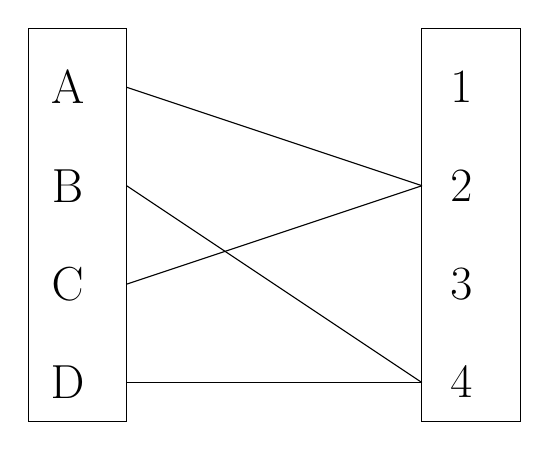
\begin{tikzpicture}
                \tikzset{every node/.style={font=\LARGE}}
                % left column (inputs)
                \draw (1.25,6.25) rectangle (2.5,1.25);
                \node at (1.75,5.5) {A};
                \node at (1.75,4.25) {B};
                \node at (1.75,3) {C};
                \node at (1.75,1.75) {D};
                % right column (outputs)
                \draw (6.25,6.25) rectangle (7.5,1.25);
                \node at (6.75,5.5) {1};
                \node at (6.75,4.25) {2};
                \node at (6.75,3) {3};
                \node at (6.75,1.75) {4};
                % mappings
                \draw (2.5,5.5) -- (6.25,4.25);
                \draw (2.5,4.25) -- (6.25,1.75);
                \draw (2.5,3) -- (6.25,4.25);
                \draw (2.5,1.75) -- (6.25,1.75);
            \end{tikzpicture}%
        }

        \\[1ex]
        Dit is een functie: elke input geeft een output.

        \vspace{1em}

% --- diagram 2 ---
        \resizebox{.6\columnwidth}{!}{%
            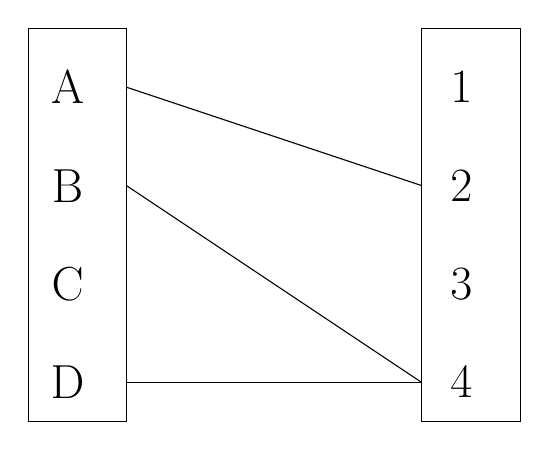
\begin{tikzpicture}
                \tikzset{every node/.style={font=\LARGE}}
                \draw (1.25,6.25) rectangle (2.5,1.25);
                \node at (1.75,5.5) {A};
                \node at (1.75,4.25) {B};
                \node at (1.75,3) {C};
                \node at (1.75,1.75) {D};
                \draw (6.25,6.25) rectangle (7.5,1.25);
                \node at (6.75,5.5) {1};
                \node at (6.75,4.25) {2};
                \node at (6.75,3) {3};
                \node at (6.75,1.75) {4};
                \draw (2.5,5.5) -- (6.25,4.25);
                \draw (2.5,4.25) -- (6.25,1.75);
                \draw (2.5,1.75) -- (6.25,1.75);
            \end{tikzpicture}%
        }

        \\[1ex]
        Ook dit is een functie, want elke input geeft een output.

        \vspace{1em}

% --- diagram 3 (not a function) ---
        \resizebox{.6\columnwidth}{!}{%
            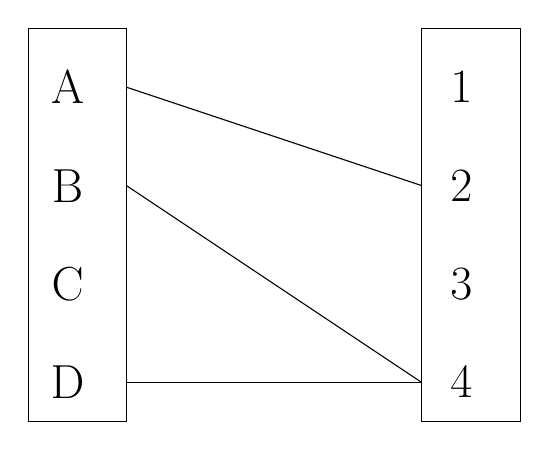
\begin{tikzpicture}
                \tikzset{every node/.style={font=\LARGE}}
                \draw (1.25,6.25) rectangle (2.5,1.25);
                \node at (1.75,5.5) {A};
                \node at (1.75,4.25) {B};
                \node at (1.75,3) {C};
                \node at (1.75,1.75) {D};
                \draw (6.25,6.25) rectangle (7.5,1.25);
                \node at (6.75,5.5) {1};
                \node at (6.75,4.25) {2};
                \node at (6.75,3) {3};
                \node at (6.75,1.75) {4};
                \draw (2.5,5.5) -- (6.25,4.25);
                \draw (2.5,4.25) -- (6.25,1.75);
                \draw (2.5,1.75) -- (6.25,1.75);
                % intentionally leave C without an outgoing line to show "not a function"
            \end{tikzpicture}%
        }

        \\[1ex]
        Dit is geen functie, want C heeft geen output, dat moet wel

        \vspace{1em}

% --- diagram 3 (not a function) ---
        \resizebox{.6\columnwidth}{!}{%
            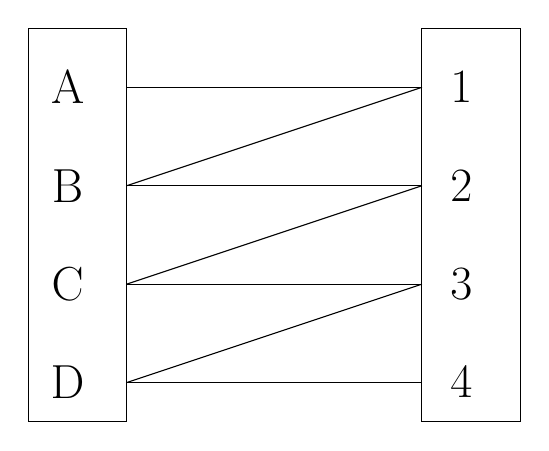
\begin{tikzpicture}
                \tikzset{every node/.style={font=\LARGE}}
                \draw (1.25,6.25) rectangle (2.5,1.25);
                \node at (1.75,5.5) {A};
                \node at (1.75,4.25) {B};
                \node at (1.75,3) {C};
                \node at (1.75,1.75) {D};
                \draw (6.25,6.25) rectangle (7.5,1.25);
                \node at (6.75,5.5) {1};
                \node at (6.75,4.25) {2};
                \node at (6.75,3) {3};
                \node at (6.75,1.75) {4};
                \draw (2.5,4.25) -- (6.25,4.25);
                \draw (2.5,1.75) -- (6.25,1.75);
                \draw (2.5,3) -- (6.25,3);
                \draw (2.5,1.75) -- (5.75,1.75);
                \draw (2.5,1.75) -- (6.25,3);
                \draw (2.5,3) -- (6.25,4.25);
                \draw (2.5,4.25) -- (6.25,5.5);
                \draw (2.5,5.5) -- (6.25,5.5);
            \end{tikzpicture}%
        }

        \\[1ex]
        Dit is geen functie, input mogen min- en maximaal 1 output hebben

    \end{multicols}


    \subsection{terminologie}
    $A$ noemen we het \textbf{domein}, en $B$ noemen we het \textbf{codomein}.
    Je kan ook meerdere argumenten meegeven: $f : A \times B \times C \longrightarrow D$
    De hoeveelheid argumenten noem je de \textbf{ariteit}.

    Als je een functie defineerd die 2 variabelen hebt, een \textbf{binaire functie} dan kan je die opeen speciale manier schrijven.
    Namelijk de functie ``+'' kan je hem tussen de variablene zetten, namelijk $A+B$ wat hetzelfde betekend als $+(A, B)$.

    \subsection{afbeelding en pre-afbeelding}
    de image van een set is je begint met een set en die zet je om naar de na-functie set.
    Deze is gedefinieerd als: $f(S) = \{f(a) : a \in S\}$.
    Te lezen als: "De set S wordt door functie f omgezet naar een nieuwe set, die bestaat uit alle outputs van f voor elk element a in S".

    De pre-image is het resultaat en die wil je dan omzetten naar het origineel.
    Deze is gedefinieerd als: $f^{-1}(T) = \{a : a \in A \land f(a) \in T\}$.
    Te lezen als: "De set T wordt door de inverse van functie f omgezet naar een nieuwe set, die bestaat uit alle inputs a in A waarvoor de output van f in T zit".

    \begin{voorbeeld}{image en pre-image}
        Dit voorbeeld met de functie: $sqrt(x)$ die inhoudt dat de output $x \times x$ bedraagt.
        We nemen ook de set $S = \{1,4,9,16\}$.\\
        Dan is de image van de set $sqrt(S)$ gelijk aan $\{1, 16, 81, 256\}$, dit is ná de functie is uitgevoerd op de input set.\\
        De Pre-image is het tegenovergestelde, die is namelijk $\{1, 2, 3, 4\}$.
        Hier kijk je naar de input set en ga je ervanuit dat de functie al is uitgevoerd en moet je dus kijken welke zet heeft dit als resultaat.
    \end{voorbeeld}

    \subsection{grafieken en identiteit functies}
    Zoals we kennen in de wiskunde van $y = 2x$, kan je een grafiek maken van de functie.
    In de functie $f : A \rightarrow B$ defineren we de subset $A \times B$ als de grafiek van f.
    Dit houdt in dat elk element in A gekoppeld is aan zijn output in B. (zoals in een xy-grafiek).
    Een graph functie is dus een verzameling van paren (a, b) waarbij a in A zit en b de output is van f(a) is.
    Zo krijg je dus de grafiek van f als: $G = \{(a, f(a)) : a \in A\}$.
    Te lezen als: "De grafiek G is de verzameling van alle paren (a, f(a)) waarbij a in A zit".
    \\\\
    De identiteit functie is een speciale functie die elk element in A koppelt aan zichzelf in B.
    Dit is dus $id : A \rightarrow A$ met $id(a) = a$ voor alle a in A.
    Dit houdt in dat de output van de functie altijd hetzelfde is als de input.

    Voor een Subset S van A, kunnen we een characteristieke functie definiëren, deze is meestal genoteerd als $\chi: A \rightarrow \{0,1\}$.
    Deze functie werkt als volgt:
    \[
        \chi(a) =
        \begin{cases}
            1 & \text{als } a \in S \\
            0 & \text{als } a \notin S
        \end{cases}
    \]
    Dit betekent dat de functie 1 teruggeeft als het element a in de subset S zit, en 0 als het element a niet in S zit.

    \subsection{injectief, surjectief en bijectief}
    Een functie kan op verschillende manieren de elementen in de sets koppelen.
    \begin{itemize}
        \item \textbf{Injectief}: Elk element in A wordt gekoppeld aan een uniek element in B.
        Dit betekent dat er geen twee verschillende elementen in A zijn die naar hetzelfde element in B wijzen.
        Dus als $f(a_1) = f(a_2)$, dan moet $a_1 = a_2$ zijn.
        \\
        De functie $f: \mathbb{R} \rightarrow \mathbb{R}$ gedefinieerd door $f(x) = 2x$ is injectief, omdat verschillende waarden van $x$ verschillende waarden van $f(x)$ opleveren, maar niet alle waarden in B worden bereikt (want, $x = 0.5$ is geen reëel getal).
        \\
        Als je een injectieve functie hebt tussen twee sets, dan kan je dat noteren als $A \preceq B$.
        Te lezen als: ``Er is een injectieve functie van A naar B.''

        \item \textbf{Surjectief}: Elk element in B wordt bereikt door ten minste één element in A.
        Dit betekent dat de functie alle elementen in B "bedient".
        Dus voor elke $b$ in B, is er minstens één $a$ in A zodat $f(a) = b$.
        \\
        De functie $g: \mathbb{R} \rightarrow \mathbb{R}$ gedefinieerd door $g(x) = x^2$ is niet surjectief, omdat negatieve waarden in B niet worden bereikt door enige waarde van $x$ in A.
        \\
        Als je een surjectieve functie hebt tussen twee sets, dan kan je dat noteren als $A \succeq B$.
        Te lezen als: ``Er is een surjectieve functie van A naar B.''
        \item \textbf{Bijectief}: De functie is zowel injectief als surjectief.
        Dit betekent dat er een één-op-één correspondentie is tussen de elementen in A en B.
        Dus elk element in A wijst naar een uniek element in B, en elk element in B wordt bereikt door precies één element in A.
        \\
        De functie $h: \mathbb{R} \rightarrow \mathbb{R}$ gedefinieerd door $h(x) = x + 1$ is bijectief, omdat elke waarde van $x$ een unieke waarde van $h(x)$ oplevert, en elke waarde in B wordt bereikt door precies één waarde van $x$.
    \end{itemize}

    Bij Bijectieve functies zijn belangrijk omdat ze een perfecte "match" tussen de twee sets creëren, wat betekent dat de lengte van beide sets gelijk is als ze eindig zijn.
    Maar dat wil je wel kunnen noteren, daarvoor is de $\simeq$ notatie.
    Dus als er een bijectie is tussen set A en set B, dan noteren we dit als $A \simeq B$.
    Dit betekent dat de cardinaliteit (grootte) van A gelijk is aan die van B.
    Dit werkt voor eindige sets, maar ook voor oneindige sets.

    Dit is niet alleen bij bijectieve functies zo, dit geldt altijd:
    \begin{itemize}
        \item De set van dagen in de week $\{Ma, Di, Wo, Do, Vr, Za, Zo\} \simeq \{1, 2, 3, 4, 5, 6, 7\}$
        \item De set van natuurlijke getallen groter dan nul $\mathbb{N}_{\eqslantgtr 0} \simeq \mathbb{N}$
    \end{itemize}

    \subsection{compositie van functies}
    Stel je hebt twee functies: $f : A \rightarrow B$ en $g : B \rightarrow C$.
    De compositie van deze twee functies, genoteerd als $g \circ f$, is een nieuwe functie die elementen van A naar C brengt door eerst f toe te passen en daarna g.
    Je leest dit dus als "g na f".
    De compositie wordt gedefinieerd als:
    \[
        (g \circ f)(a) = g(f(a))
    \]
    voor alle $a$ in A.
    Dit betekent dat je eerst de functie f toepast op het element a om een element in B te krijgen, en vervolgens pas je de functie g toe op dat resultaat om een element in C te krijgen.

    Het is goed om te weten dat als beide functies injectief zijn, dan is hun compositie ook injectief.
    Als beide functies surjectief zijn, dan is hun compositie ook surjectief.
    En als beide functies bijectief zijn, dan is hun compositie ook bijectief.

    \begin{voorbeeld}{Bijectieve functies en compositie}
        Stel je hebt de functie $f(x) = 2x + 3$, deze is bijectief omdat elke waarde van x een unieke waarde van f(x) oplevert, en elke waarde in de codomein wordt bereikt door precies één waarde van x (ervan uitgaande dat de codomein alle reële getallen bevat).
        Als je wilt bewijzen dat $f$ bijectief is, kun je de volgende stappen volgen:
        Je splitst de functie op in twee delen: eerst $g(x) = 2x$ en daarna $h(x) = x + 3$.
        Beide functies zijn bijectief:
        \begin{itemize}
            \item $g(x) = 2x$ is injectief omdat verschillende waarden van x verschillende waarden van g(x) opleveren, en het is surjectief omdat elke waarde in de codomein wordt bereikt door precies één waarde van x.
            \item $h(x) = x + 3$ is ook injectief en surjectief om dezelfde redenen.
        \end{itemize}
        Omdat zowel $g$ als $h$ bijectief zijn, is hun compositie $f(x) = h(g(x)) = 2x + 3$ ook bijectief.
    \end{voorbeeld}

    \newpage

    \section{Relaties}

    \subsection{properties of realtions}
    \begin{itemize}
        \item Reflexiviteit: als $R(x,x)$ voor alle $x$, bijvoorbeeld gelijkheid
        \item Symetrie: als $R(x,y) \implies R(y,x)$, bijvoorbeeld gelijkheid, of 'is sibling of (de broer van mijn zus ben ik)'
        \item Asymetrie: als $R(x,y) \implies \neg R(y,x)$
        \item Transitief: als $R(x,y) \land R(y,z) \implies R(x,z)$, bijvoorbeeld gelijkheid $3=1+2$ en $1+2=1+1+1$ dus $3=1+1+1$
    \end{itemize}

    \subsection{relaties defineren}

    \subsection{Equivalentie klasse}
    Als je bepaalde sets als "gelijk" wil beschouwen dan kan je dit gebruiken.
    Je kan dan bijvoorbeeld zeggen: auto's zijn gelijk als het model en merk het zelfde zijn, kleur maakt niet uit.
    Of $1/2$ is gelijk aan $2/4$, het detail dat ze niet 1 op 1 hetzelfde zijn maakt niet meer uit.
    Ze zijn niet gelijk, maar wel equivalent.

    \subsection{partities}
    Als je een set A heb met een eindig aantal partities $A_1, A_2, A_3, ..., A_n$
    Dan is elke partitie $A_i \cap A_j = \emptyset$ wanneer $i \neg j$.
    En bij elkaar $A_1 \cup A_2 \cup ... \cup A_n = A$.
    Oftewel, elke parties heeft elementen die niet in een andere set zitten.
    en als je ze weer samenvoegt, dan krijg je de originele set A weer.

    \ruleline{Alles hierboven is stof voor de eerste midterm}

    \section{Inductie}
    Elke inductie is omschreven met 3 stappen:
    \begin{enumerate}
        \item De \textbf{base case}, die verteld dat er sommige elementen in een set zit
        \item De \textbf{inductieove case}, die verteld dat als een bepaalde waarde in de set zit, dat die waarde er ook bij moet. Bijv. je hebt een set met 1 iemand, en dan voeg je alle mensen toe die hij/zij kent, en die kennen ook weer mensen die je dan toe voegt etc.
        \item De \textbf{external clause}, die geeft aan dat elementen die niet toegevoegd zijn door case 1 en 2 niet worden toegevoegd.
    \end{enumerate}
    \\\\

    \begin{multicols}{2}

    \noindent Voor de set $\mathbb{N}$ natuurlijke nummers, gaat het als volgt:
    \begin{itemize}
        \item $0 \in \mathbb{N}$.
        \item voor elke $n \in \mathbb{N}$, voeg $(n + 1) \in \mathbb{N}$.
        \item Er zijn geen andere getallen uit $\mathbb{N}$.
    \end{itemize}

    \noindent Voor de set even natuurlijke nummers, gaat het als volgt:
    \begin{itemize}
        \item $0 \in \mathbb{N}$.
        \item voor elke $n \in \mathbb{N}$, voeg $(n + 2) \in \mathbb{N}$, wanneer $(n - 2) \in \mathbb{N}$, waar $n \neq 0$ bestaat
        \item Er zijn geen andere getallen uit $\mathbb{N}$.
    \end{itemize}

    \end{multicols}

    \subsection{Backus-Naur Form}
    Dit is een hele korte manier om inductie te schrijven:
    $w::= \epsilon | 0w | 1w$, hier staat dat $\epsilon$ is een word w, dan is 0w een word in de set én 1w is ook een word in de set.
    Dus dan kan je bijv. $w = {0}$ nemen, dan krijg je na een iteratie $w = {0, 10, 00}$




\end{document}